\documentclass[12pt]{paper}

\usepackage[margin=1in]{geometry}
\usepackage{tikz}
\usepackage{graphicx}
%\usepackage{Schwieg}

\usepackage{amsmath}
\usepackage{bm}
\usepackage{amsthm}
\usepackage{mathtools}
\usepackage{bbm}


\DeclareMathOperator{\diam}{diam}
\DeclareMathOperator{\interior}{int}
\DeclareMathOperator{\close}{cl}

\newcommand{\met}[1]{d \left ( #1 \right )}
\newcommand{\brak}[1]{ \left [ #1 \right ] }
\newcommand{\cbrak}[1]{ \left \{ #1 \right \}}
\renewcommand{\vec}[1]{ \bm{ #1 }}
\newcommand{\abs}[1]{\left \lvert #1 \right \rvert}
\newcommand{\seq}[1]{{\left \{ #1 \right \}}}
\newcommand{\conj}[1]{ \overline{ #1 } }
%\newcommand{\close}[1]{ \bar{ #1 } }
\newcommand{\set}[1]{\left \{ #1 \right \}}
\newcommand{\Lim}{\lim\limits}
\newcommand{\compose}{\circ}
\newcommand{\inv}[1]{{#1}^{-1}}
\newcommand{\compl}[1]{{#1}^{c}}



\newcommand{\setR}{ \mathbb{R} }
\newcommand{\setQ}{ \mathbb{Q} }
\newcommand{\setZ}{ \mathbb{Z} }
\newcommand{\setN}{ \mathbb{N} }

\newcommand{\plim}{ \overset{p}{\to} }
\newcommand{\mean}[2][N]{ \overline{ #2 }_{#1}}
\newcommand{\exV}[1]{\mathbb{E} \left [ #1 \right ]}
\newcommand{\Vari}[1]{\mathbb{V} \left ( #1 \right )}
\newcommand{\est}[2][N]{ \widehat{ #2 }_{#1}}
\newcommand{\indicate}[1]{ \mathbbm{1}_{\{#1\}}}
\newcommand{\convDist}{ \overset{d}{\to}}
\newcommand{\unif}{\emph{U}}
\newcommand{\normal}{\mathcal{N}}

\DeclarePairedDelimiter{\ceil}{\lceil}{\rceil}
\DeclarePairedDelimiter{\floor}{\lfloor}{\rfloor}
\DeclarePairedDelimiter{\norm}{\lVert}{\rVert}

\newtheorem*{definition}{Definition}
\newtheorem{theorem}{Theorem}[section]
\newtheorem{question}{Question}
\newtheorem*{answer}{Answer}

\title{Price Theory 1 - Problem Set 1 - Question 1}
\author{Samuel Barker \and
  Timothy Schwieg \and
  Rafeh Qureshi \and
  Daniel Noriega \and
Ana Vasilj}

\begin{document}

\maketitle

\section*{Part A}

Consider a world where there are three agents, consumers, land-owners
and firms. Labor and Capital are freely mobile and can move between regions.

Assume that the firms face a production function exhibiting constant
returns to scale. Suppose that no firm, consumer, or land-owner has any
market power. Assume that all consumers have the same strictly quasi-concave
utility function and that the firm's production function is strictly
quasi-concave. Assume that each region has a fixed quantity of land
$\overline{X}$. 

One important notion is that the regions in this problem vary solely
by the quality of land between them. By examining how the factor
prices and quantities vary with the different quality levels, we
answer how they vary with the different regions.

\subsection*{Consumers}

Consumers value their leisure time as well as their consumption of the
single good produced in this world: $Y$. For a given time period, they
must choose their labor/leisure trade-off as well as the region in
which they are inhabiting. As consumption of good $Y$ is the same
across regions as well as leisure, the region can only affect their
wage. The consumers value only the good and their leisure. Their
utility function is modeled as: $U( Y, Le)$. A consumer's only income
source is working; the consumer's income for region $i$ is $w_i \ell_i$
where $\ell$ is the amount of hours they work.

Immediately we can notice that the only part of this decision where
the region chosen by the consumer is relevant is in his wage. His
leisure and purchasing power of $Y$ are unaffected by where he lives,
except indirectly through the wage. This is mathematically equivalent
to the consumer first selecting the region with the highest wage, and
then choosing his leisure time based on that wage. For an equilibrium
to be supported he must be indifferent between living between all
regions, as labor is freely mobile.

This implies that the only equilibrium that can be supported is the
equilibrium where all the regions pay the same wage. If there
was some region with a higher wage, then no consumer would want to
live elsewhere, and firms in that specific region could lower
their wage and make strictly more profit. Likewise a no wage could be
below either, as they would attract no workers.

Under these conditions, the consumer solves this problem: 
\begin{align*}
  \max_\ell \quad& U( w \ell, 1 - \ell)\\
          &\text{s.t.} \ell \in [0,1]
\end{align*}

This generates a perfectly elastic supply curve at the price $w$ for
labor. Each consumer works for $\ell$ units of time, as all consumers
have the same utility function, and therefore work the same amount of
time $\ell$, the hours worked by each consumer are equal across all
consumers. We shall assume that the consumer is never in a
backwards-bending portion of his labor supply, i.e.
$\frac{\partial \ell}{\partial w} > 0$.


\subsection*{Firms}
Suppose there are many firms in each region of the economy all using
the same production function, and producing output. Assume there
exists a capital market operating in the background at the nationwide
level. This leads to an equilibrium rental rate of capital $r$. As
there are many small firms without market power, they must be price
takers in the market, and suppose that capital is homogeneous and the
market is competitive.

It is equivalent to solve the firm's problem with $Q$ as some
exogenous variable, as the only difference between the regions is the
value of $Q$. Then we can look at how each firm behaves at different
values of $Q$ to determine how firms in different regions act.

From the discussion on the consumer, it is known that every firm will
have to offer the same wage to each worker regardless of region that
the firm is located in.

The firms face a production function of
\begin{equation*}
  Y = F( T, K, L)
\end{equation*}
Where $T = QX$, is the ``efficiency units'' of the land, $K$ is the
capital employed, and $L$ is the amount of labor employed.
This function exhibits constant returns to scale. Note that each unit
of ``efficiency units'' is homogeneous, and the firm faces a constant
price for purchasing effective land.

Consider the cost function of this firm:
\begin{align*}
  C(y,t,w,r) = &\min_{T,K,L} tT + wL + rK\\
  &\text{s.t.} F(T,K,L) = y
\end{align*}

This is equivalent to the Hicksian system for a utility function of
$F(T,K,L)$. So the cost function is concave. We also know that the
solution is characterized by a tangency of the expenditure with the
isoquant. Since the production function exhibits CRS, its level curves
all have the same slope following a ray out of the origin. So if we
can find one tangency for a given output $y$, then the optimal
inputs for any other output must lie along the ray.

This tells us that the expansion path, or the choice of inputs to meet
larger and larger outputs follows along a line. This means that as you
scale $y$, each of the inputs scales with each other by the same
amount, increasing the cost by that scale as well. As the firm sells
at a constant price, it must earn zero profit.

Following these assumptions are the standard competitive assumptions
implied by profit maximization.
\begin{align*}
  F_L(T,K,L) = w\\
  F_K(T,K,L) = r\\
  F_X(QX,K,L)Q = t
\end{align*}

That is, that the price of each factor input equals the benefit of
each factor input. These functions give rise to three factor demand
equations. $X^{*}, L^{*}, K^{*}$ which are the optimal amounts of each
of the factor inputs for a given set of input prices and quality $Q$.

\subsection*{Land Owners}

Each land owner has $\overline{X}$ quantity of land where the quality of each
piece of land is given by $Q$. This can be thought of us each region
having a different quantity of homogeneous land. Since there is
nothing else that the land-owners can do with their land, they face no
opportunity cost of renting the land to the firms. They are willing to
accept any price for their land.

This leads to a perfectly inelastic supply at the maximum amount of
land supplied. The land-owner has no monopoly power in the market.
If the land owner were to attempt to restrict his output, he would
have no affect on the price. He simply faces a price and tries to sell as
much of his land as possible. As a result supply is fixed at the
amount of land in the region. This gives us perfectly inelastic demand
at the total land.

$$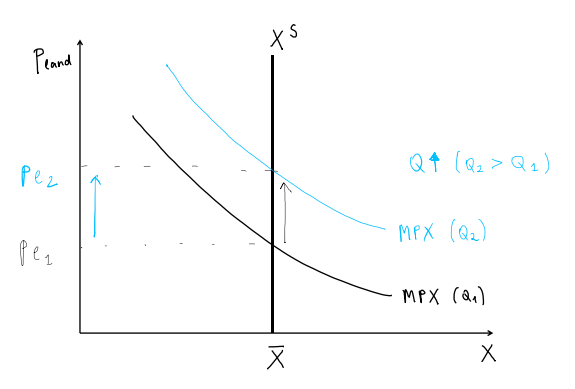
\includegraphics[width=0.5\textwidth]{fixedLand.png}$$


\subsection*{Equilibrium}

In Equilibrium, there will be no excess demand or supply in terms of
labor, capital, land or the good $Y$. This gives us several conditions
that must hold:

$$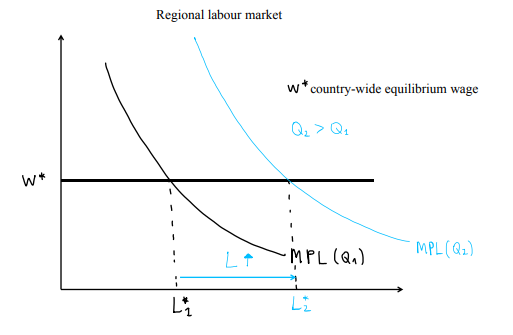
\includegraphics[width=0.5\textwidth]{regionalLabor.png}$$

The first condition is that the wages must be equal across the
different regions. The rental rate is equal between the different
regions as well, as a result of the capital market being exogenous and
open to the entire country.The rental rate of capital is determined by
the returns to capital in all regions, so it fixes the marginal
productivity of capital for all firms to be constant.

$$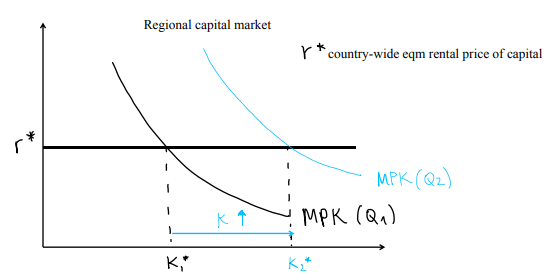
\includegraphics[width=0.55\textwidth]{regionalCapitalMarket.png}$$

Each region has $\overline{X}$ land, thus the effective quantity
of land is fixed per region. Equilibrium in the land market will occur
where $MPT = MPX Q$ intersects this perfectly inelastic supply. Since
our production function is CRS, then $MPX$ is constant as the optimal
level of inputs are all linear in $Q$. Therefore the land price will
be linear in $Q$.

Since supply of land is perfectly inelastic, an increase in $Q$ must
lead to an increase in the effective land used by the firm. Therefore
it must be the case that the firm is producing more output. This can
be seen by considering the conditional factor demand equations. The
factor demand for land at a given level of output for the first
quantity of effective land is optimal, so the only way that the high
quantity is optimal is if more output is produced. If output
increases, we have shown that the optimal path is linear. This tells
us that factor quantities vary exactly with the quality of the land as
well. That is: $Q_2L_1^{*} = Q_1L_2^{*}$ and
$Q_2 K_1^{*} = Q_1 K_2^{*}$. So the ratio of labor to capital is
fixed, and the ratio of land to labor and capital is decreasing.

\section*{Part b - Individuals Require Land}

Now consumers must consume a fixed amount of land when they work in a
region. Assume that per region there is a cost of renting given by
$R_i$. To work in a particular region, consumers now have income: $w_i
L - R_i$.

The land-owners no longer have a perfectly inelastic supply curve.  In
this world they face a price of renting their land to the firms -
renting it to a consumer. For an equilibrium to occur, the land-owner
should be indifferent between renting out his land and selling it to a
consumer. Note that for a fixed amount of land that a consumer
requires (normalized to $1$), the price of renting this land is $Q$
units of effective land that could be used by the firm. Thus the
rental price of houses must be increasing in $Q$. Indifference implies
that $R(Q) = t(Q) = MPX Q$. Note that $MPX$ will not, in general, be
constant along the output path anymore. Thus rents will not be linear
in $Q$ anymore.

Consumers must also be indifferent between regions. They now face
rents that are different between regions. Their budget line in each region,
adjusted by the rent cost must lie tangent to the same indifference
curve as the budget line of all other regions. This determines the
wage increase that must exist to compensate for the rental cost. Any
increase in the rental cost must be accompanied by an increase in the
wage for this indifference to occur. We can notice that by our
assumptions, individuals will always choose to work more as rent
increases. This tells us that the hours worked by an individual:
$\ell(Q)$ is increasing in $Q$. This function $\ell$ must be concave as
well, as from above $0$ rent, the individual will choose to increase
his work load by less because the income effect is becoming stronger
as he gains income.

$$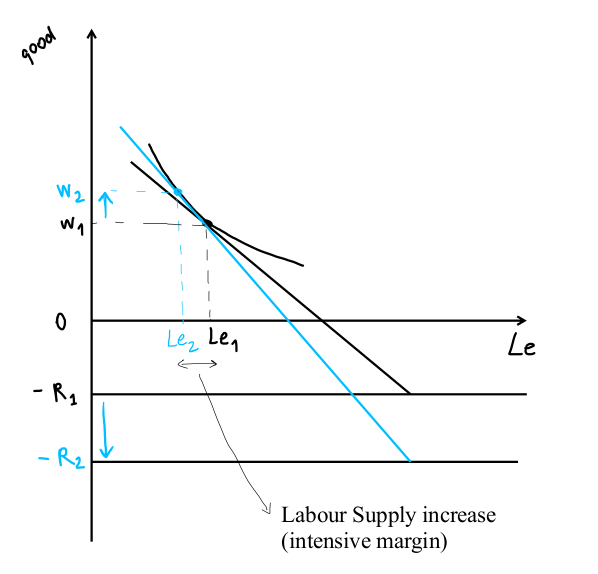
\includegraphics[width=0.5\textwidth]{laborleisurePlot.png}$$

As we see an increase in the quality of the available land, the cost
of renting out a unit of that land to a consumer increases, as it
could be used as more effective land to the firm. For benefits to
equal out the costs, the benefit for the firm, $MPX$ must
increase. The cost of renting, $R(Q)$ increases in $Q$. This increase
in the price of the land to the owner though is larger than the
increase in the quality of the land, as some of this land must also be
rented out to the new labor required for the increased
production. This added labor compounds the increase in $MPX$. This
tells us that $X^{*}$, the optimal amount of land rented to firms,
decreases. We must give some land over to the labor required to help
our more effective land, and this is costly. However $QX^{*}$ must
still be non-decreasing. If it were decreasing, it would not be
possible for the old value of $QX^{*}$ to be optimal. Not all of the
``new'' land that is generated by the increase in quality is rented to
labor, so the remaining land goes to the firm. This means that the
firm is using more effective land, even if less land is being rented
to the firm.

With the increase in $Q$ there is an increase in effective land and
labor used by the firm. These are both complements to capital, so the
productivity of capital has increased. Without changes, the benefit of
capital is above its exogenous cost of $r$. In order to drive $MPK$
down to the level where $MPK = r$ the firm needs to use more
capital. The increased capital has the added effect of raising $MPX$
and $MPL$.

$MPL$ is increased by the increased amount of $QX^{*}$ and the
increased amount of $K^{*}$, but decreased by the increased amount of
$L^{*}$. However the total effect must be positive. We can note that
$MPL = w(Q)$ and that wages are an increasing function of Rental
prices. Since renting to consumers is more expensive as quality rises,
wages must rise as well. It would be a contradiction for rental rates
to rise and the overall effect on wages to be negative.

We know that the total amount of land allocated to firms and rented to
consumers must be equal to the total land. Note that since $L^{*}$ is
the man-hours worked, and $\ell(Q)$ is the hours worked of a consumer,
$\frac{L^{*}}{\ell(Q)}$ is the number of workers.
\begin{align*}
  \frac{L^{*}}{\ell(Q)} + X^{*} = \overline{X}\\
  L^{*} = \ell(Q) ( \overline{X} - X^{*})
\end{align*}

We may note that since $\ell(Q)$ is increasing in $Q$ and $X^{*}$ is
decreasing in $Q$, then the labor supply $L^{*}$ is increasing in
$Q$. This is intuitive, as quality growth makes the already allocated
land more effective, so some of it will be substituted over to labor
such that the marginal benefit is equal to the marginal cost.

$$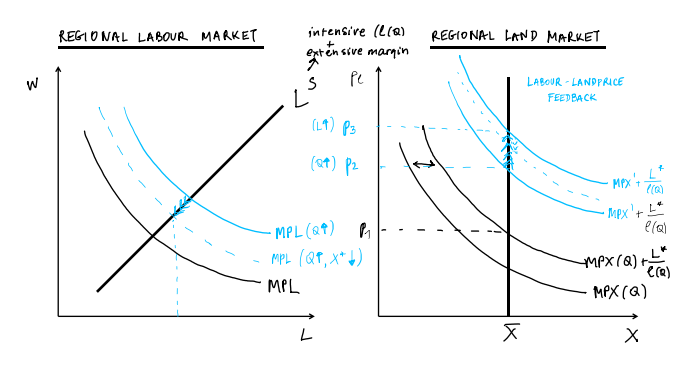
\includegraphics[width=1.0\textwidth]{part2LandLabor.png}$$


In equilibrium the factor prices for land and labor have increased,
and capital has remained constant. We may note that the price of land
is increasing at a rate that is super-linear in $Q$, as land becomes
more scarce. While wages are increasing, there is downward pressure on
them caused by the increased labor when $Q$ increases, so the
magnitude depends on the magnitudes of the complementary factors.

Since the factor inputs of land and labor are increasing in $Q$,
capital has become relatively cheaper to purchase. So Capital
production is convex in $Q$. As $Q$ gets larger, we want more capital,
and it becomes relatively less expensive, driving the ratio of capital
upwards over labor and land. This can be thought of as a short-run
effect where land and labor are restricted by total quantity of land
in a region, so they cannot be as sensitive to a change in $Q$ as they
were in part (a). To deal with this problem, the firm substitutes
extra capital to deal with the increased costs of using land and
capital. This tells us that the ratio of land to capital is decreasing
in $Q$, and labor to capital is decreasing in $Q$ as well. The ratio
of land to labor is decreasing as well as $X^{*}$ is decreasing in $Q$
and $L^{*}$ is increasing in $Q$.

\section*{Part c}

In the second model, the land-owner faces a choice to rent to the firm
and to a consumer. As $Q$ increases, the cost of renting to an
individual becomes more expensive, so he must receive an increased
benefit for there to be an equilibrium. In the original model this
choice does not exist, so he requires less incentive to be willing to
sell his land. This enforces that the prices of land are increasing by
more in the second model than they are in the first model.

This effectively is a standard equilibrium notion. There is a higher
opportunity cost of renting to the firm in the second model, as he
does not earn rents from renting to consumers, so there must be a
higher benefit in order for there to be an equilibrium.
\end{document}

%  LocalWords:  isoquants
